\begin{frame}[t]{
\includegraphics[width=0.3cm]{circle1} Global Flux Quadrature  with WENO approximation} 
\MyLogoa

 We seek solutions of the hyperbolic system of balance laws

\begin{equation}
	\partial_tU+\partial_x F(U)=  S(U)\partial_xH   \nonumber
	\vspace{0.25cm}
\end{equation}


{\bf \textsf{Approach 1.}\footnote{M. Ciallella, D. Torlo, MR, Arbitrary High Order WENO Finite Volume Scheme with Flux Globalization for Moving Equilibria Preservation,  {\it J.Sci.Comp.} 96, 2023 }} 

\only<1-2>{ \begin{equation*} 
 \dfrac{d\overline{U}_i}{dt} + \dfrac{1}{\Delta x} \left( \widehat{G}_{i+1/2} - \widehat{G}_{i-1/2}   \right)   = 0  \nonumber
 \vspace{0.35cm}
\end{equation*}}
 
 \only<2>{
 
 \begin{enumerate}
 \item  Reconstruct  WENO polynomials  ${\color{red}U_i(x)}$
 
 \vspace{0.175cm}
 
 \item  Compute  cell averaged source primitive $ \overline{R}_i =R_{i-1/2}^+ - \sum_q \omega_q  \int_{x_{i-1/2}}^{x_q} S({\color{red}U_i(x)},\varphi(x)) dx$
 
  \vspace{0.1cm}
  
   \item  Compute  cell averaged fluxes  $ \overline{F}_i =  \sum_q \omega_q F({\color{red}U_i(x_q)},\varphi(x_q)) dx$
 
  \vspace{0.175cm}
  
 \item  Reconstruct  WENO polynomials  $G_i(x)= (F+R)_i(x)$ 
 
  \vspace{0.175cm}
  
 \item  Compute upwind fluxes $\widehat{G}_{i+1/2} = (A^+A^{-1})_{i+1/2} G_{i}(x_{i+1/2}) + (A^-A^{-1})_{i+1/2} G_{i+1}(x_{i+1/2})$
 \end{enumerate}
 }

\only<3>{
\vspace{-0.5cm}
\begin{center}
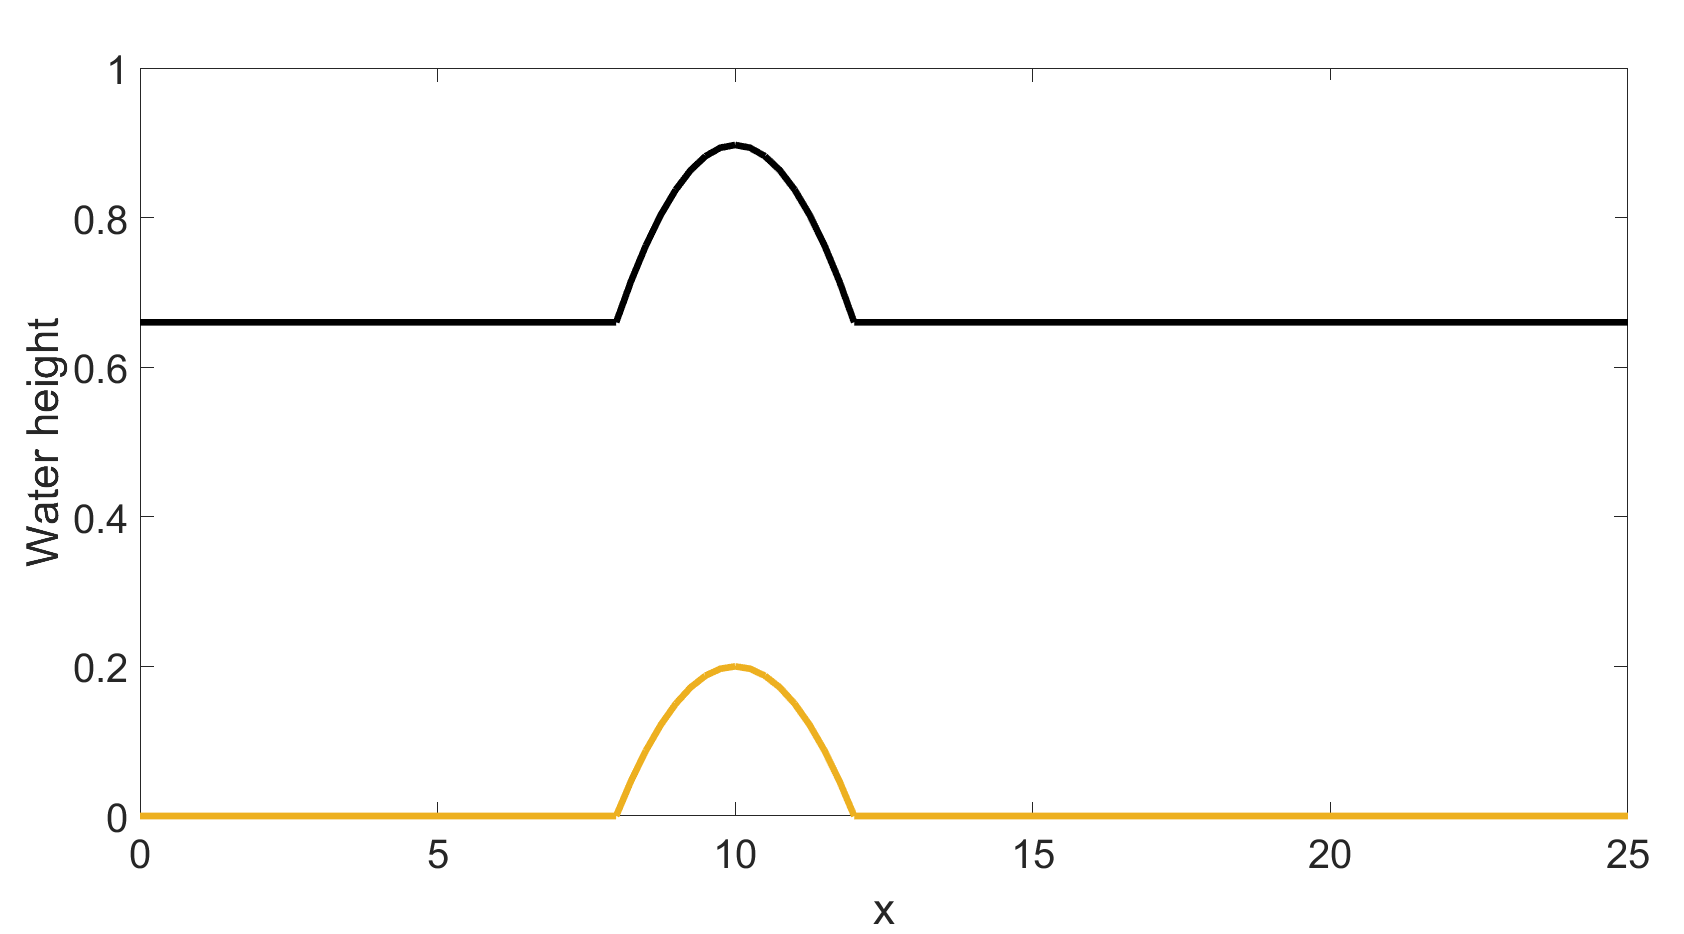
\includegraphics[width=3.5cm,height=1.25cm]{./height_supercrit}\\
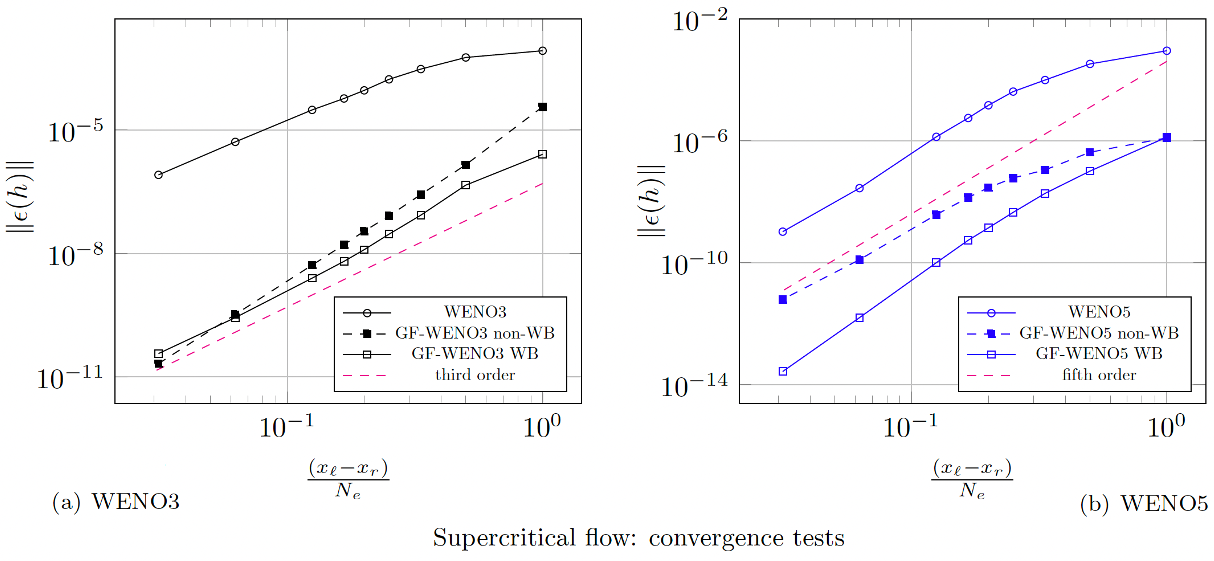
\includegraphics[width=0.6\textwidth]{./GF-FV-WENO-conv}
\end{center}
} 

\only<4>{
{\sf\small Small perturbation of steady state}\\
\begin{center}
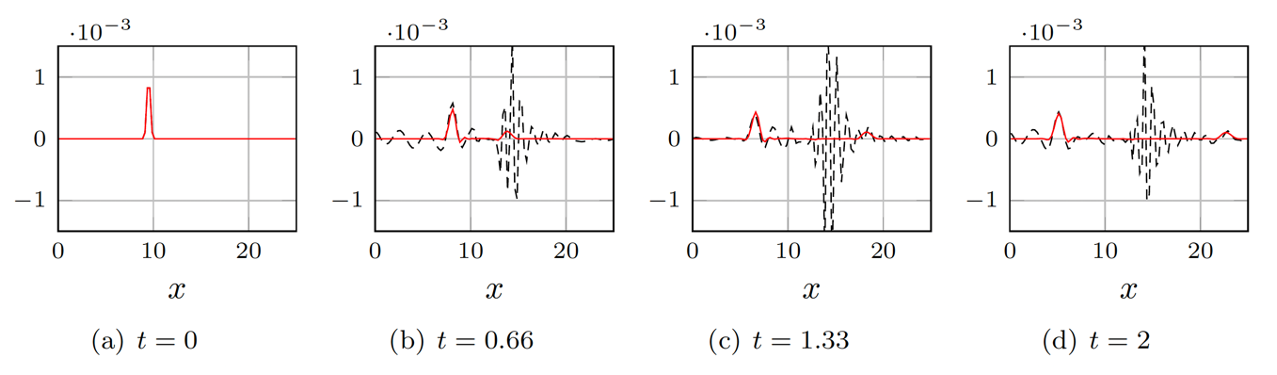
\includegraphics[width=0.9\textwidth]{./GF-WENO-FV-pert} 
\end{center}
} 


\only<5>{
\begin{enumerate}
\item[\textcolor{mblue1}{\Large\checkmark}] \textcolor{black}{No a-priori knowledge of equilibrium, all steady states!}  

\vspace{0.2cm}

\item[\textcolor{mblue1}{\Large\checkmark}] \textcolor{black}{No need of compute the solution of the Cauchy problem .. (maybe for initialization)}  

\vspace{0.2cm}

\item[\textcolor{mblue1}{\Large\checkmark}]  \textcolor{black}{Considerable accuracy enhancements at steady state (3 to 4 orders of magnitude)}

\vspace{0.2cm}

\item[\textcolor{red}{\Large$\times$}]  \textcolor{black}{No super convergence} 

\vspace{0.2cm}

\item[\textcolor{red}{\Large$\times$}]  \textcolor{black}{Very hard to charcterize the steady state and generate one }
\end{enumerate}

\begin{flushright}
$ \overline{R}_i =R_{i-1/2}^+ - \sum_q \omega_q  \int_{x_{i-1/2}}^{x_q} S({\color{red}U_i(x)},\varphi(x)) dx$
\end{flushright}
}




\end{frame}
 
 
 \begin{frame}[t]{
\includegraphics[width=0.3cm]{circle1} Global Flux Quadrature  with WENO approximation} 
\MyLogoa

 We seek solutions of the hyperbolic system of balance laws

\only<1-3>{\begin{equation}
	\partial_tU+\partial_x F(U)=  S(U)\partial_xH   \nonumber
	\vspace{0.25cm}
\end{equation}}

\only<4-6>{\begin{equation}
	\partial_tU+\partial_x \dfrac{U^2}{2}=  S(U) \partial_xH     \nonumber
	\vspace{0.25cm}
\end{equation}}
\only<7->{\begin{equation}
	\partial_t\bigg[\begin{array}{c} h\\hu\end{array}\bigg]+\partial_x\bigg[\begin{array}{c} hu\\hu^2 + gh^2/2\end{array}\bigg]=  - \bigg[\begin{array}{c} 0\\h\end{array}\bigg] b'(x)   \nonumber
%	\vspace{0.25cm}
\end{equation}}

{\bf \textsf{New approach}} 


\only<1-2>{ \begin{equation*} 
 \dfrac{d U_i}{dt} + \dfrac{1}{\Delta x} \left( \widehat{G}_{i+1/2} - \widehat{G}_{i-1/2}   \right)   = 0  \nonumber
 \vspace{0.35cm}
\end{equation*}}
 
 \only<2>{
 
 \begin{enumerate}
 \item  \sout{Reconstruct  WENO polynomials  $U_i(x)$}
 
 \vspace{0.15cm}
 
 \item  Compute  nodal  source primitive $ R_i =R_{i-1} - \Delta x \sum_q \omega_q  S(U_{i-q},\varphi(x_{i-q}))$
 
  \vspace{0.15cm}
  
   \item  \sout{Compute  cell averaged fluxes  $ \overline{F}_i =  \sum_q \omega_q F({\color{red}U_i(x_q)},\varphi(x_q)) dx$}

  \vspace{0.15cm}
    
 \item  Reconstruct  WENO polynomials  $G_{i+1/2}^{\pm}(x)= (F+R)^{\pm}_{i+1/2}(x)$ 
 
  \vspace{0.15cm}
  
 \item  Compute upwind fluxes $\widehat{G}_{i+1/2} = P^+_{i+1/2} G^-_{i+1/2}(x_{i+1/2}) + P^-_{i+1/2} G_{i+1/2}^+(x_{i+1/2})$
 \end{enumerate}
 }

\only<3>{
\begin{block}{Main result}
 {\bf Proposition} (Discrete steady state). {\it     The  WENO-FD scheme with  global flux quadrature 
 preserves exactly \underline{continuous} discrete  steady states $U^*_i =U(F_i)$ with $F$  obtained by integrating the ODE
 $$
 F' = S(U(F)) \partial_x H 
 $$ 
using the  multi-step ODE integrator with weights $\{\omega_q\}_{q\ge 0}$  %\footnote{See e.g.  Theorem 7.10 in Hairer, Wanner and Norset, Solving Ordinary Differential Equations I., Springer 1993}:   
on   spatial slabs of size $\hh$. \\[2.pt]

If $U(F)$ is a one to one mapping,    $U^*(x)$  
 verifies the  consistency estimates of the multi-step scheme.
 }  
 
 \end{block}
 
 \vspace{0.5cm}
 
 \begin{flushright}
{\rm Multi-step schemes so far: Adams methods AB$n$ and AM$n$}
\end{flushright}
} 

 \only<4>{
For $S(U)=U^2$ and $H(x)=x$ exact steady state $u=e^x$ \\[10pt]


\begin{minipage}{0.5\textwidth}
\centering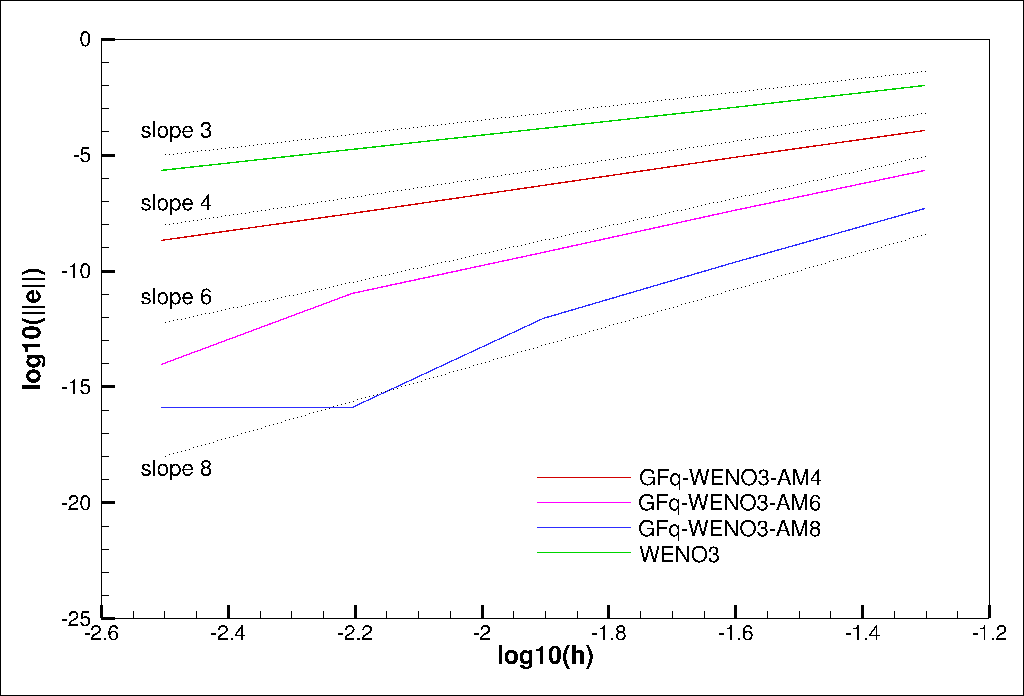
\includegraphics[width=0.8\textwidth]{../figs/WENO-FD/figures/Burgers/convergence_steady/convburg-weno3} 
\end{minipage}\hfill
\begin{minipage}{0.5\textwidth}
\centering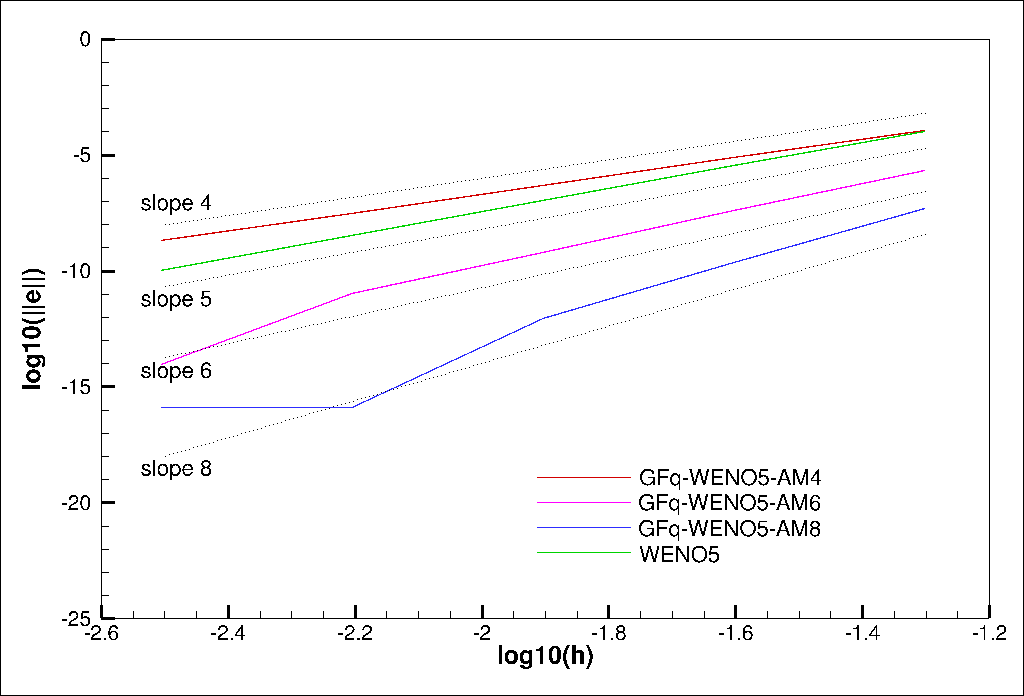
\includegraphics[width=0.8\textwidth]{../figs/WENO-FD/figures/Burgers/convergence_steady/convburg-weno5}
\end{minipage}
} 

\only<5>{
For $s(U)=U^2$ and $\varphi=x+100\sin x$   \\[5pt]


\begin{minipage}{0.5\textwidth}
\centering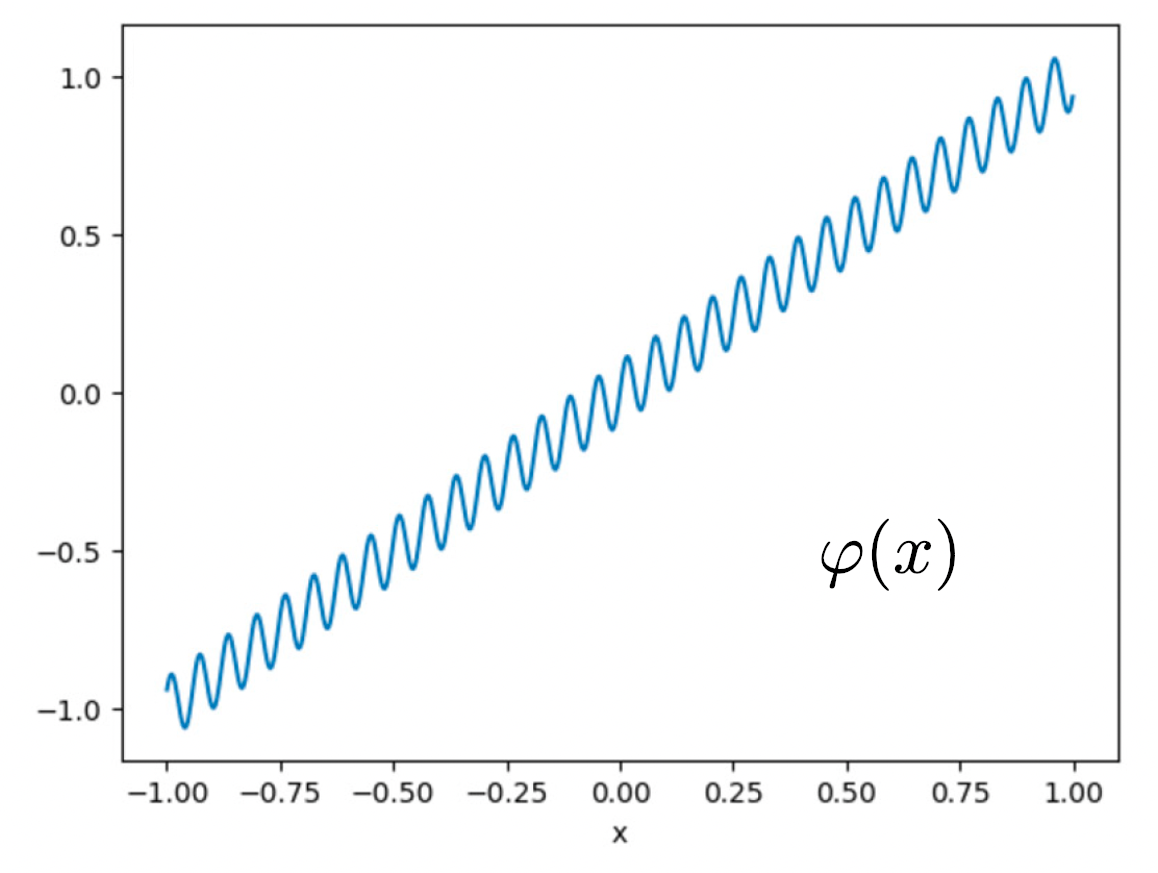
\includegraphics[width=0.8\textwidth]{../figs/WENO-FD/figures/Burgers/perturbations/oscillation} 
\end{minipage}\hfill
\begin{minipage}{0.5\textwidth}
\centering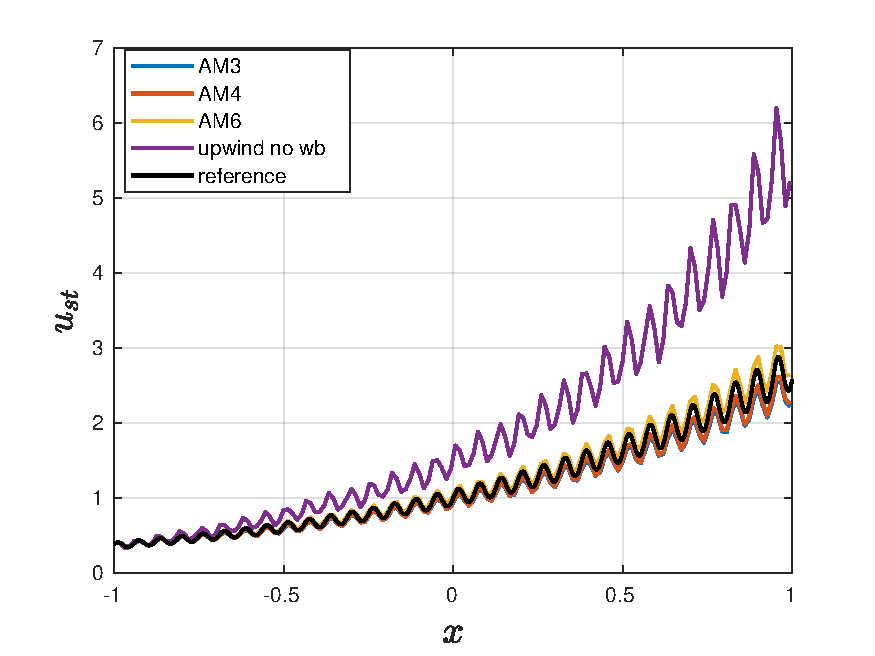
\includegraphics[width=0.85\textwidth]{../figs/WENO-FD/figures/Burgers/perturbations/weno3_AM_stationary_n150} 
\end{minipage}
} 


\only<6>{
For $S(U)=u^2$ and $H=x+100\sin x$ + top hat of perturbation $\delta u=0.2\chi_{[-0.7,-0.5]}$    \\[5pt]


\begin{minipage}{0.5\textwidth}
\centering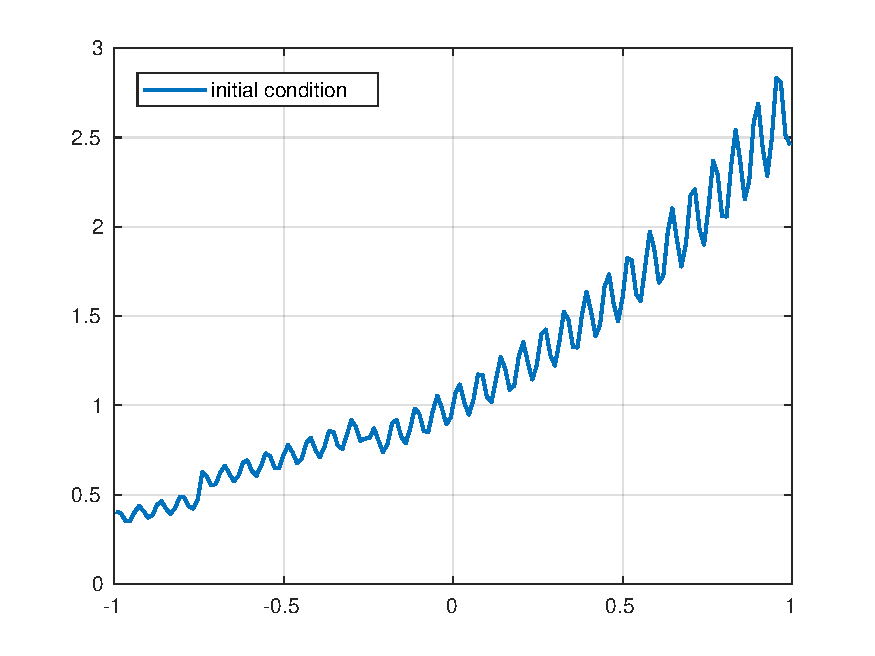
\includegraphics[width=0.8\textwidth]{../figs/WENO-FD/figures/Burgers/perturbations/initial_cond_DISC_n150} 
\end{minipage}\hfill
\begin{minipage}{0.5\textwidth}
\centering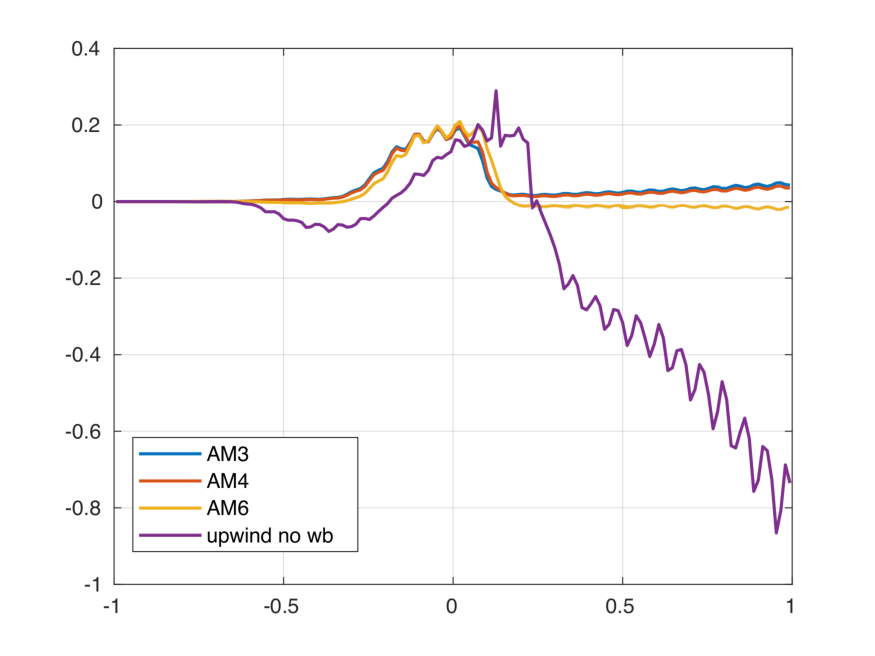
\includegraphics[width=0.85\textwidth]{../figs/WENO-FD/figures/Burgers/perturbations/weno3_AM_DISC_n150} 
\end{minipage}
} 
\only<7>{
\begin{minipage}{0.4\textwidth}
Supercritical flow on a smooth hump\\
\centering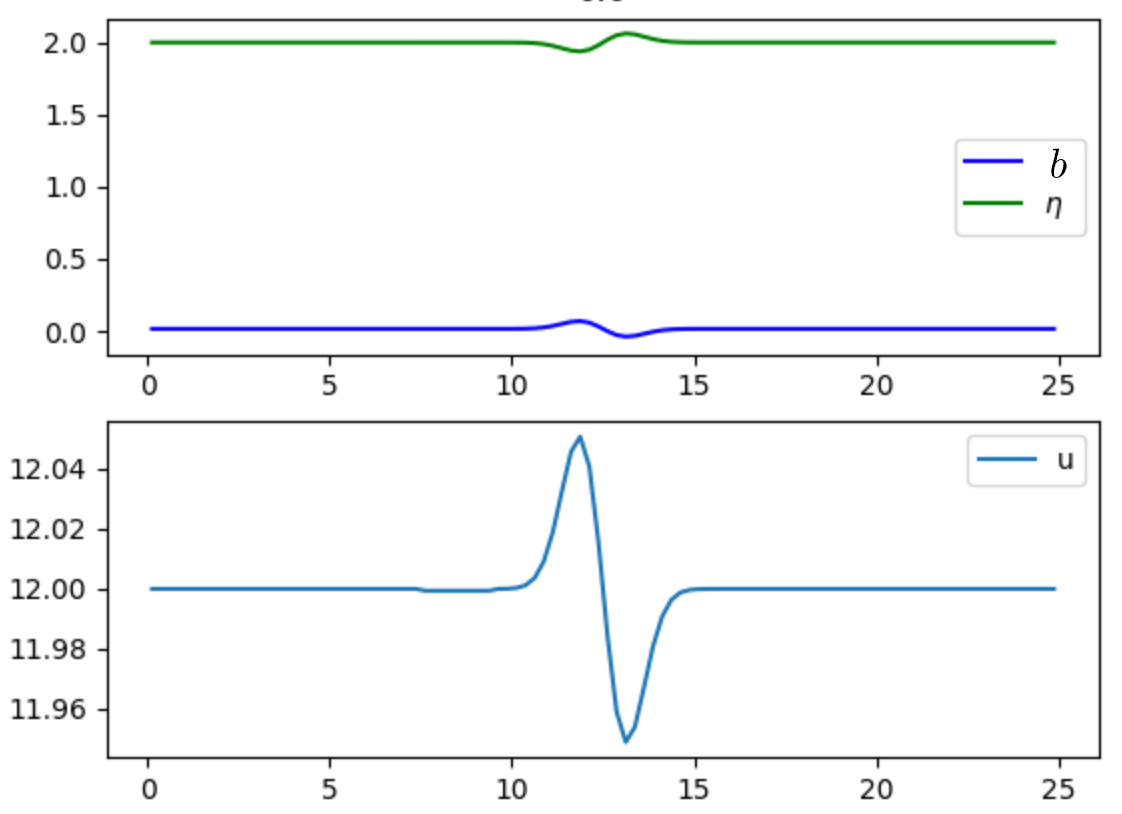
\includegraphics[width=\textwidth]{../figs/WENO-FD/figures/SW/Subcritical/super-ini} 
\end{minipage}\hfill
\begin{minipage}{0.6\textwidth}
\centering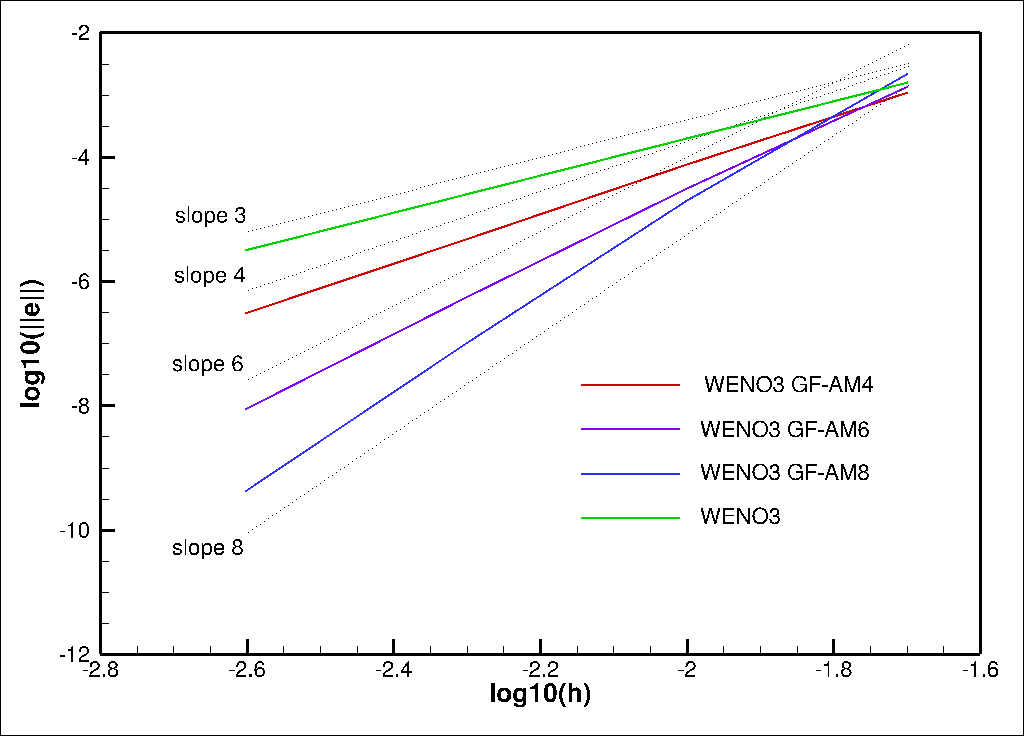
\includegraphics[width=0.8\textwidth]{../figs/WENO-FD/figures/SW/Subcritical/conv} 
\end{minipage}
}

\only<8>{
\begin{minipage}{0.5\textwidth}
\centering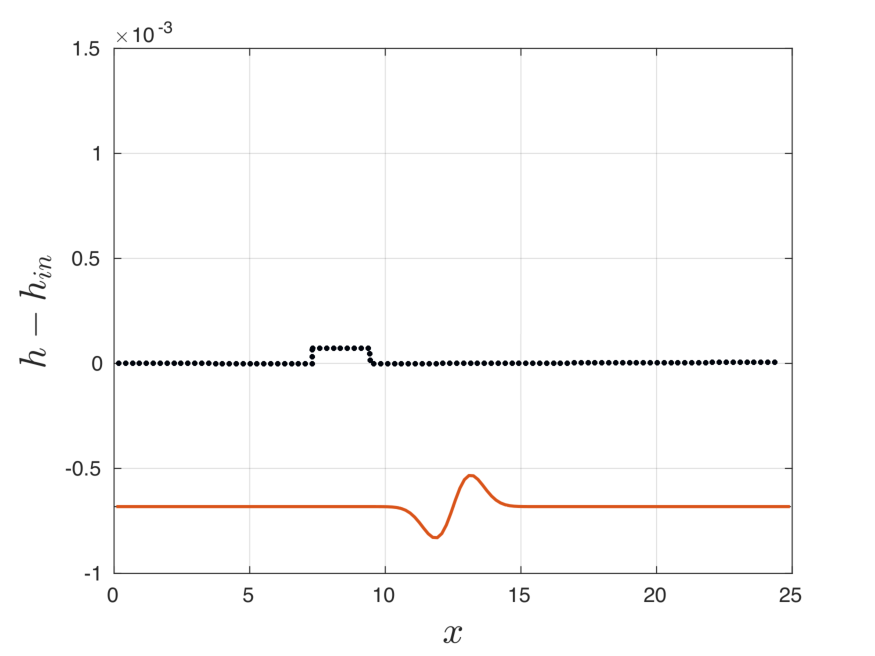
\includegraphics[width=0.9\textwidth]{../figs/WENO-FD/figures/SW/perturbations/weno3_sup_DISCsmall_n100_error_ini}
\end{minipage}\hfill
\begin{minipage}{0.5\textwidth}
\centering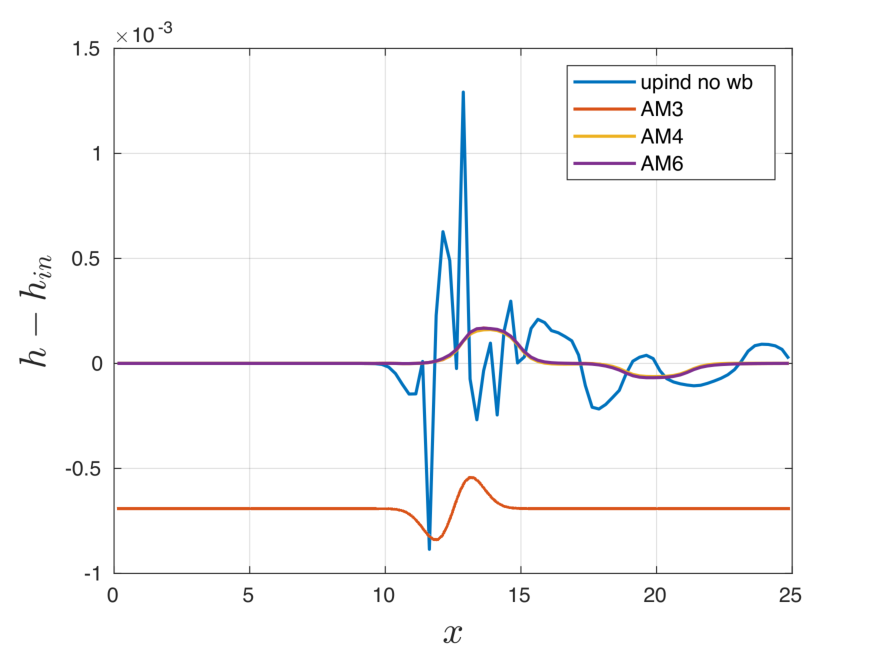
\includegraphics[width=0.9\textwidth]{../figs/WENO-FD/figures/SW/perturbations/weno3_sup_DISCsmall_n100_error_h} 
\end{minipage}
}


\only<9>{
\begin{minipage}{0.5\textwidth}
\centering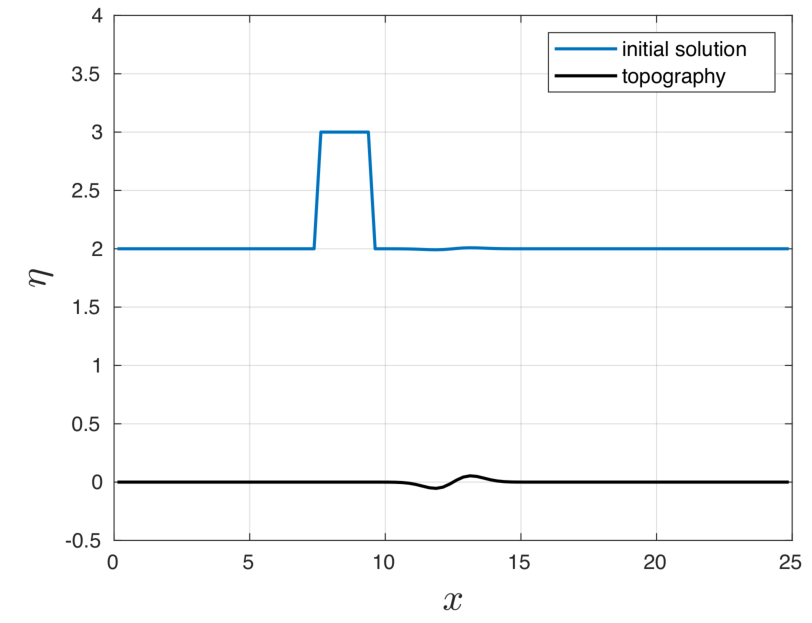
\includegraphics[width=0.9\textwidth]{../figs/WENO-FD/figures/SW/perturbations/initial_discbig}
\end{minipage}\hfill
\begin{minipage}{0.5\textwidth}
\centering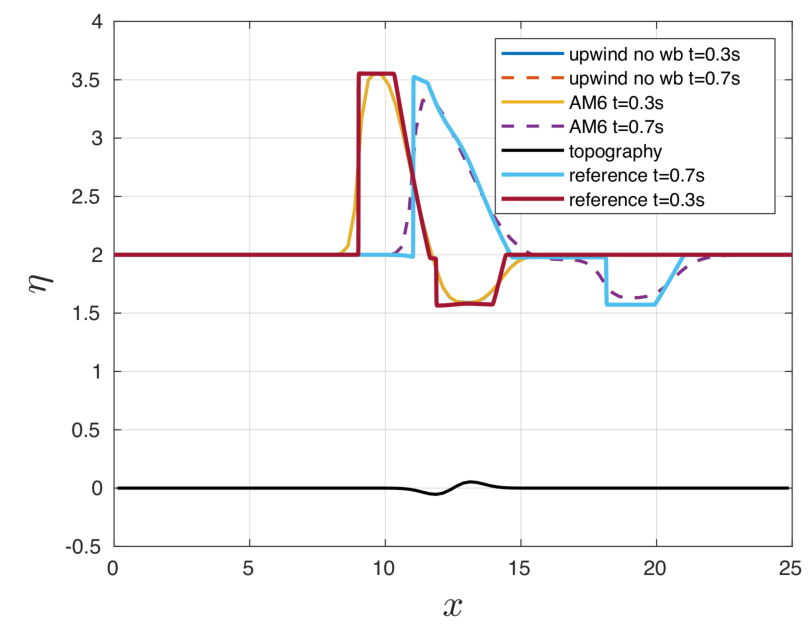
\includegraphics[width=0.9\textwidth]{../figs/WENO-FD/figures/SW/perturbations/weno3_evolution_upAM61} 
\end{minipage}
}


\only<10>{

\vspace{0.5cm}

\begin{enumerate}
\item[\textcolor{mblue1}{\Large\checkmark}] \textcolor{black}{No a-priori knowledge of equilibrium, all steady states!}    

\vspace{0.2cm}

\item[\textcolor{mblue1}{\Large\checkmark}] \textcolor{black}{No need of compute the solution of the Cauchy problem .. (maybe for initialization)}  

\vspace{0.2cm}

\item[\textcolor{mblue1}{\Large\checkmark}]  \textcolor{black}{Convergence at steady state arbitrarily accurate by changing ODE weights} 

\vspace{0.2cm}

\item[\textcolor{mblue1}{\Large\checkmark}]   \textcolor{black}{Discrete initial state can be generated}

\vspace{0.2cm}

\item[\textcolor{red}{\Large$\times$}]   \textcolor{black}{Non-compact quadrature }
\end{enumerate}

}

\end{frame}
% 